
\scsubsection{Введение в язык линейного представления баз знаний ostis-систем}
\label{intro_scs}

\begin{SCn}

\scnsectionheader{\currentname}

\scnstartsubstruct

\scnsegmentheader{Первый сегмент Введения в язык графического представления баз знаний ostis-систем}

\scnstartsubstruct

\scnheader{Введение в язык графического представления баз знаний ostis-систем}
\scnidtf{Введение в SCs-код}
\scnreltovector{конкатенация сегментов}{Первый сегмент Введения в SCs-код;Описание Алфавита SCs-кода;Описание sc.s-разделителей;Описание sc.s-ограничителей;Описание sc.s-предложений;Описание Ядра SCs-кода и различных направлений его расширения}

\scnheader{SCs-код}
\scnidtf{Semantic Code string}
\scnidtf{Язык линейного представления баз знаний ostis-систем}
\scnidtf{Множество всевозможных текстов SCs-кода}
\scnidtf{Тексты SCs-кода}	
\scnaddlevel{1}
\scniselement{имя собственное}
\scnaddlevel{-1}
\scnidtf{текст SCs-кода}	
\scnaddlevel{1}
\scniselement{имя нарицательное}
\scnaddlevel{-1}
\scnidtf{sc.s-текст}
\scniselement{линейный язык}
\scnrelfrom{алфавит}{Алфавит SCs-кода}
\scnrelfrom{разделители}{sc.s-разделитель}
\scnrelfrom{ограничители}{sc.s-ограничитель}
\scnrelfrom{предложения}{sc.s-предложение}
\scnrelfrom{идентификаторы}{sc.s-идентификатор}
\scnrelfrom{неоднозначные обозначения описываемых сущностей}{неоднозначное sc.s-изображение sc-элемента}
\scnexplanation{Множество линейных текстов (sc.s-текстов), каждый из которых состоит из предложений (sc.s-предложений), разделенных друг от друга двойной точкой с запятой (разделителем sc.s-предложений). При этом sc.s-предложение представляет собой последовательность sc.s-идентификаторов, являющихся именами описываемых сущностей и разделяемых между собой различными sc.s-разделителями и sc.s-ограничителями}

\scnheader{sc.s-идентификатор}
\scnidtf{идентификатор, построенный по правилам SCs-кода}
\scnidtf{имя, построенное по правилам SCs-кода, обозначающее (идентифицирующее) соответствующую сущность, а так же одновременно идентифицирующее синонимичный этому имени sc-элемент, обозначающий ту же сущность, что и указанное имя}

\scnaddlevel{1}
	\scnidtf{строковый идентификатор}
	\scnsubset{идентификатор}
	\scnexplanation{обозначение описываемой сущности, структура которого в формальных языках однозначно соответствует этой сущности}
\scnaddlevel{-1}
\scnsubdividing{
простой sc.s-идентификатор\\
\scnaddlevel{1}
\scnidtf{атомарный sc.s-идентификатор}
\scnidtf{sc.s-идентификатор некоторого sc-элемента, в состав которого другие sc.s-идентификаторы (sc.s-идентификаторы других sc-элементов) не входят}
\scnidtf{простой (атомарный) внешний строковый идентификатор sc-элемента}
\scnaddlevel{-1}
;sc.s-выражение\\
\scnaddlevel{1}
\scnidtf{неатомарный sc.s-идентификатор}
\scnidtf{sc.s-идентификатор, представляющий собой в общем случае иерархическую конфигурацию sc.s-идентификаторов, связываемых между собой соответствующими sc.s-разделителями и sc.s-ограничителями}
\scnaddlevel{-1}
}

\scnheader{неоднозначное sc.s-изображение sc-элемента}
\scnidtf{условное обозначение не именуемой (неидентифицируемой) сущности}
\scnsuperset{sc.s-коннектор}
\scnaddlevel{1}
    \scnidtf{неоднозначное sc.s-изображение sc-коннектора, являющееся также одновременно одним из видов sc.s-разделителей}
    \scnsubset{sc.s-разделитель}
\scnaddlevel{-1}
\scnsuperset{неоднозначное sc.s-изображение sc-узла}
\scnaddlevel{1}
    \scnsuperset{условное обозначение неименуемого множества sc-элементов}
    \scnaddlevel{1}
        \scnexplanation{условное обозначение неименуемого множества sc-элементов в SCs-коде представляется строкой из двух символов -- левой фигурной скобки и правой фигурной скобки. В SCs-коде, это соответствует кружочку с точкой внутри}
    \scnaddlevel{-1}
    \scnsuperset{условное обозначение неименуемого кортежа sc-элементов}
    \scnaddlevel{1}
        \scnexplanation{В SCs-коде такое обозначение представляется двух-символьной строкой левой угловой скобки и правой угловой скобки}
    \scnaddlevel{-1}
	\scnsuperset{условное обозначение неименуемого файла-экземпляра ostis-системы}
	\scnaddlevel{1}
		\scnexplanation{В SCs-коде такое обозначение представляется двух-символьной строкой левой квадратной скобки и правой квадратной скобки}
	\scnaddlevel{-1}
	\scnsuperset{условное обозначение не именуемого файла-класса ostis-системы}
	\scnaddlevel{1}
		\scnexplanation{В SCs-коде такое обозначение представляется трех-символьной строкой левой квадратной скобки, вертикальной черты (***), правой квадратной скобки}
	\scnaddlevel{-1}
\scnaddlevel{-1}
	
\scnendstruct

\scnsegmentheader{Описание Алфавита SCs-кода}
\scnstartsubstruct

\scnheader{Алфавит SCs-кода}
\scnidtf{Алфавит символов SCs-кода}
\scnidtf{множество символов SCs-кода}
\scnidtf{символ, используемый в текстах SCs-кода}
\scnreltoset{объединение}{символ, используемый в sc.s-разделителях;символ, используемый в sc.s-ограничителях;символ, используемый в простых sc.s-индетификаторах}

\scnheader{символ, используемый в sc.s-разделителях}
\scnhaselements{\textit{подчеркнутый пробел};\textit{дефис};\textit{запятая};\textit{пробел};\textit{точка};\textit{точка с запятой};\textit{двоеточие};\textit{“мячик”};\textit{знак равенства}}
\scnhaselement{знак инцидентности правого sc-коннектора}
\scnaddlevel{1}
\scneqfileclass{|-}
\scnaddlevel{-1}
\scnhaselement{знак инцидентности левого sc-коннектора}
\scnaddlevel{1}
\scneqfileclass{-|}
\scnaddlevel{-1}
\scnhaselement{знак инцидентности входящей sc-дуги справа}
\scnaddlevel{1}
\scneqfileclass{|<}
\scnaddlevel{-1}
\scnhaselement{знак инцидентности входящей sc-дуги слева}
\scnaddlevel{1}
\scneqfileclass{>|}
\scnaddlevel{-1}

\scnheader{символ, используемый в sc.s-разделителях}
\scnsuperset{символ, используемый в sc,s-коннекторах}
\scnaddlevel{1}
\scnhaselements{\scnfileclass{$\in$};\scnfileclass{$\ni$};\scnfileclass{$\notin$};\scnfileclass{$\not \ni$};\scnfileclass{***};\scnfileclass{***};\scnfileclass{$\sim$};\textit{знак подчеркивания};\textit{знак тире};\textit{знак равенства};\scnfileclass{>};\scnfileclass{<};\scnfileclass{$\subseteq$};\scnfileclass{$\supseteq$};\scnfileclass{$\subset$};\scnfileclass{$\supset$};\scnfileclass{$\leq$};\scnfileclass{$\geq$};\textit{двоеточие}}
\scnaddlevel{-1}

\scnheader{символ, используемый в sc.s-разделителях}
\scnhaselement{вертикальная черта}
\scnhaselement{двойная вертикальная черта}
\scnaddlevel{1}
\scnidtf{знак операции конкатенации}
\scnaddlevel{-1}
\scnhaselement{знак операции объединения множеств}
\scnaddlevel{1}
\scnidtf{$\cup$}
\scnaddlevel{-1}
\scnhaselement{знак пересечения множеств}
\scnaddlevel{1}
\scnidtf{$\cap$}
\scnaddlevel{-1}
\scnhaselement{знак операции разности множеств}
\scnaddlevel{1}
\scnidtf{$\backslash$}
\scnaddlevel{-1}
\scnhaselement{знак операции сложения}	
\scnaddlevel{1}
\scnidtf{+}
\scnaddlevel{-1}
\scnhaselement{знак операции умножение}	
\scnaddlevel{1}
\scnidtf{*}
\scnaddlevel{-1}
\scnhaselement{знак операции вычитания}	
\scnaddlevel{1}
\scnidtf{‑}
\scnaddlevel{-1}

\scnheader{символ, используемый в sc.s-ограничителях}
\scnhaselement{прямые кавычки}
\scnaddlevel{1}
\scnidtf{"}
\scnaddlevel{-1}
\scnhaselement{левая круглая скобка}
\scnaddlevel{1}
\scnidtf{(}
\scnaddlevel{-1}
\scnhaselement{правая круглая скобка}
\scnaddlevel{1}
\scnidtf{)}
\scnaddlevel{-1}
\scnhaselement{левая фигурная скобка}
\scnhaselement{правая фигурная скобка}
\scnhaselement{левая угловая скобка}
\scnhaselement{правая угловая скобка}
\scnhaselement{левая квадратная скобка}
\scnhaselement{правая квадратная скобка}
\scnhaselement{косая черта}
\scnhaselement{звездочка вверху}
\scnhaselement{левая цитатная кавычка}
\scnhaselement{правая цитатная кавычка}

\scnheader{символ, используемый в простых sc.s-идентификаторах}
\scnsuperset{буква Русского языка}
\scnaddlevel{1}
\scnnote{и заглавная, и строчная}
\scnaddlevel{-1}
\scnsuperset{буква Английского языка}	\scnaddlevel{1}
\scnnote{и заглавная, и строчная}
\scnaddlevel{-1}
\scnsuperset{цифра}
\scnsuperset{спецсимвол, используемый в простых sc.s-идентификаторах}
\scnaddlevel{1}
\scneqtoset{знак подчеркивания;тире;дефис;запятая;	пробел;точка;двойная точка;прямая кавычка;звездочка вверху;крестик вверху;апостроф;круглая скобка}
\scnaddlevel{-1}

\scnendstruct \scnsourcecomment{Завершили Описание Алфавита SCs-кода}

\scnsegmentheader{Описание sc.s-разделителей}
\scnstartsubstruct

\scnheader{sc.s-разделитель}	\scnidtf{разделитель, используемый в sc.s-текстах}
\scnsubdividing{sc.s-разделитель, используемый в простых sc.s-идентификаторах;sc.s-разделитель, используемый в sc.s-выражениях\\
\scnaddlevel{1}
    \scnsuperset{точка с запятой}
    \scnaddlevel{1}
        \scneqfileclass{;}
    \scnaddlevel{-1}
    \scnsuperset{"мячик"}
    \scnaddlevel{1}
        \scneqfileclass{$\bullet$}
    \scnaddlevel{-1}
\scnaddlevel{-1}
;sc.s-разделитель, используемый для структуризации sc.s-предложений\\
\scnaddlevel{1}
    \scnsuperset{sc.s-коннектор}
    \scnsuperset{sc.s-разделитель, изображающий связь инцидентности sc-элементов}
    \scnsuperset{двоеточие}
    \scnaddlevel{1}
        \scneqfileclass{:}
        \scnnote{Разделяет ***}
    \scnaddlevel{-1}
\scnaddlevel{-1}
;sc.s-разделитель sc.s-предложений\\
\scnaddlevel{1}
    \scneqfileclass{;;}
    \scnidtf{двойная точка с запятой}
\scnaddlevel{-1}
}

\scnheader{sc.s-разделитель, используемый в простых sc.s-идентификаторах}
\scnsuperset{пробел}
\scnaddlevel{1}
    \scnnote{используется в качестве разделителя между словами, входящими в состав простого sc.s-иден\-ти\-фи\-ка\-то\-ра}
\scnaddlevel{-1}
\scnsuperset{подчеркнутый пробел}
\scnsuperset{запятая}
\scnaddlevel{1}
    \scnnote{используется в качестве разделителя между некоторыми словами, входящими в состав простого sc.s-иден\-ти\-фи\-ка\-то\-ра}
\scnaddlevel{-1}
\scnsuperset{точка}
\scnaddlevel{1}
    \scneqfileclass{.}
    \scnnote{используется в конце аббревиатур, например, в инициалах}
\scnaddlevel{-1}
\scnsuperset{двойная точка}
\scnaddlevel{1}
    \scneqfileclass{..}
    \scnnote{используется в качестве разделителя между содержательно разными частями простого sc.s-иден\-ти\-фи\-ка\-то\-ра, состоящего из нескольких фраз}
\scnaddlevel{-1}
\scnsuperset{двойная точка}
\scnaddlevel{1}
    \scneqfileclass{-}
    \scntext{примеры использования}{sc-текст; sc.s-разделитель}
\scnaddlevel{-1}

\scnheader{sc.s-коннектор}
\scnidtf{изображение sc-коннектора во внешнем тексте SCs-кода или SCn-кода}
\scnsubset{sc.s-разделитель}
\scnnote{типология sc.g-коннекторов и, тем более, sc-коннекторов, т.к. она она учитывает устоявшиеся традиции изображения связок целого ряда конкретных отношений}
\scnsubdividing{ориентированный sc.s-коннектор;неориентированный sc.s-коннектор}
\scnsubdividing{sc.s-коннектор, соответствующий sc.g-дуге принадлежности\\
\scnaddlevel{1}
    \scnrelfrom{таблица}{Таблица. Алфавит sc.s-коннекторов, соответствующих sc.g-дугам принадлежности}
\scnaddlevel{-1}
;sc.s-коннектор, соответствующий sc.g-коннектору, который не является sc.g-дугой принадлежности\\
\scnaddlevel{1}
    \scnaddhind{-1}
    \scnrelfrom{таблица}{Таблица. Алфавит sc.s-коннекторов, соответствующих sc.g-коннекторам, которые не являются sc.g-дугами принадлежности}
\scnaddlevel{-1}
}

\scnheader{Таблица. Алфавит sc.s-коннекторов, соответствующих sc.g-дугам принадлежности}
\scneqfile{\\
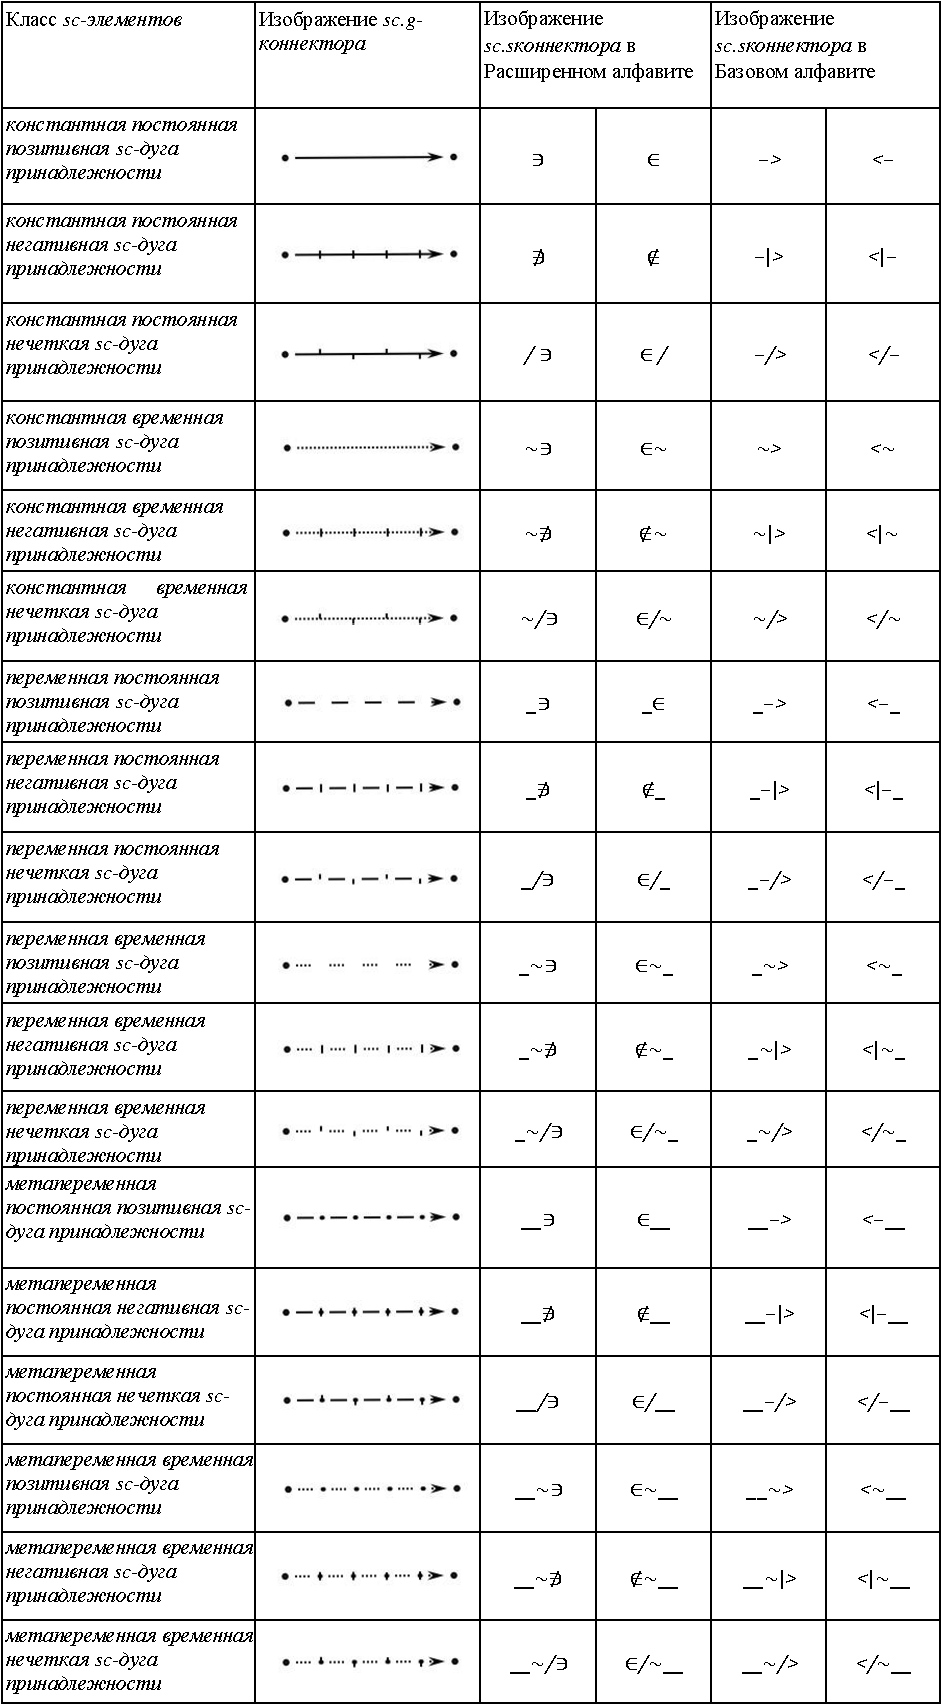
\includegraphics[width=1\linewidth]{figures/intro/scs_membership_connectors.pdf}\\
}

\scnheader{Таблица. Алфавит sc.s-коннекторов, соответствующих sc.g-коннекторам, которые не являются sc.g-дугами принадлежности}
\scneqfile{\\
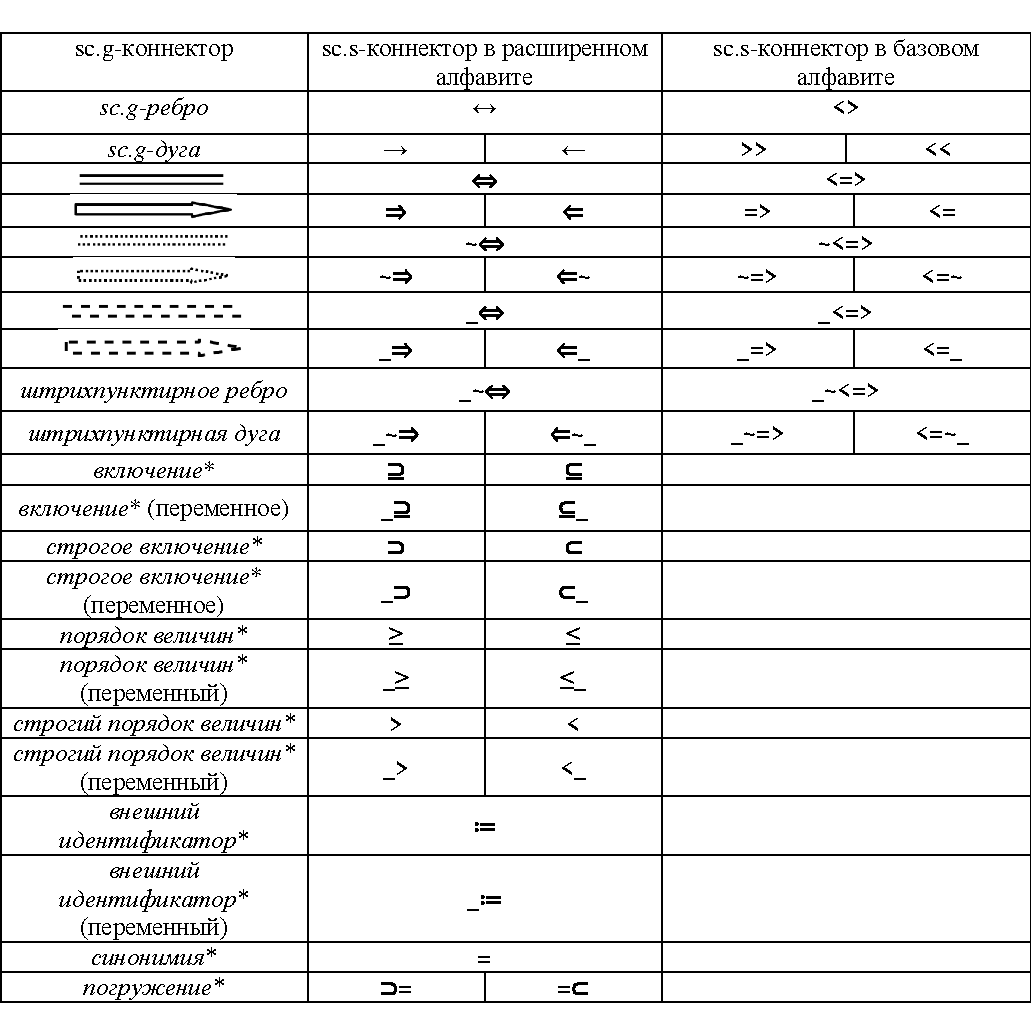
\includegraphics[width=1\linewidth]{figures/intro/scs_non_membership_connectors.pdf}\\
}

\scnheader{знак равенства}
\scneqfileclass{=}
\scnidtf{связь синонимии идентификаторов}
\scnnote{знак равенства является sc.s-разделителем двух sc.s-идентификаторов, которые идентифицируют (именуют) одну и ту же сущность и, соответственно, являются внешними идентификаторами* (внешними уникальными изображениями) одного и того же sc-элемента. При этом из указанных двух sc.s-идентификаторов чаще всего один является простым sc.s-идентификатором, а второй -- sc.s-выражением. Реже оба эти sc.s-идентификатора являются sc.s-выражениями. И совсем редко оба они являются простыми sc.s-идентификаторами. Последнее обозначает то, что оба эти sc.s-идентификатора являются основными внешними идентификаторами* одного и того же sc-элемента. Пример:

SC-код = sc.s-текст;;

Здесь первый sc.s-идентификатор является именем собственным, а второй -- именем нарицательным.

При трансляции sc.s-текста в SC-код знаку равенства на некотором этапе может быть поставлено в соответствие sc-ребро, принадлежащее отношению синонимии* sc-элементов, идентифицируемых sc.s-идентификаторами, связанными знаком равенства. Но на последующем этапе указанное sc-ребро \uline{удаляется}, а связанные им sc-элементы \uline{склеиваются}. Таким образом sc-ребро, принадлежащее отношению синонимии* sc-элементов, т.е. имеет не только денотационную, но и операционную семантику.}

\scnheader{знак равенства с включением}
\scneq{{\normalfont(}\scnfileclass{$\supset$=} $\cup$ \scnfileclass{=$\subset$}{\normalfont)}}
\scnidtf{изображение sc-дуги, принадлежащей отношению погружения*, связывающей два sc-узла, обозначающих sc-тексты, первый из которых является погружающим, а второй (в который указанная sc-дуга входит) является погружаемым, вводимым в состав первого sc-текста}
\scnnote{sc-дуга, принадлежащая отношению погружения*, интерпретируется как команда погружения одного sc-текста в состав другого. При выполнении этой команды (1) все sc-элементы погружаемого sc-текста становятся элементами, принадлежащими погружающему sc-тексту, (2) все синонимичные sc-элементы, оказавшиеся в составе погружающего sc-текста, склеиваются, (3) sc-узел, обозначающий погружаемый sc-текст, а так же спецификация этого sc-текста (включая перечень всех его sc-элементов) погружается в историю эволюции базы знаний вместе со спецификацией события погружения рассматриваемого sc-текста в состав базы знаний.}

\scnheader{{\normalfont(}знак равенства $\cup$ знак равенства с включением{\normalfont)}}
\scnnote{указанные sc.s-коннекторы отличаются от остальных sc.s-коннекторов тем, что они и соответствующие им sc-коннекторы (sc-ребра, принадлежащих отношению синонимии sc-элементов и sc-дуги, принадлежащие отношению погружения одного sc-текста в состав другого) имеют не только денотационную, но и операционную семантику, т.к. являются командами склеивания и командами погружения.}

\scnheader{sc.s-разделитель, изображающий связь инцидентности sc-элементов}
\scnsubdividing{знак инцидентности “правого” sc-коннектора\\
\scnaddlevel{1}
\scnidtf{знак инцидентности sc-коннектора, sc.s-идентификатор которого находится справа}
\scneqfileclass{|-}
\scnaddlevel{-1}
;знак инцидентности “левого” sc-коннектора\\
\scnaddlevel{1}
\scnidtf{знак инцидентности sc-коннектора, sc.s-идентификатор которого находится слева}
\scneqfileclass{-|}
\scnaddlevel{-1}
;знак инцидентности входящей sc-дуги справа\\
\scnaddlevel{1}
\scnidtf{знак инцидентности sc-дуги, sc.s-идентификатор который находится справа}
\scneqfileclass{|<}
\scnaddlevel{-1}
;знак инцидентности входящей sc-дуги слева\\
\scnaddlevel{1}
\scnidtf{знак инцидентности sc-дуги, sc.s-идентификатор который находится слева}
\scneqfileclass{>|}
\scnaddlevel{-1}}
\scnexplanation{На множестве sc-элементов задано бинарное ориентированное отношение инцидентности sc-элементов, а так же подмножество этого отношения -- отношение инцидентности входящих sc-дуг, каждая пара которого связывает sc-дугу с тем sc-элементом, в который она входит.
В SC-коде sc-коннекторы могут соединять между собой не только sc-узел с sc-узлами, но и sc-узел с sc-коннектором и даже sc-коннектор с sc-коннектором. В последнем случае, указывая инцидентность sc-коннекторов, необходимо уточнить, какой из них является соединяемым (связываемым), а какой-соединяющим (связующим). Поэтому отношение инцидентности, заданное на множестве sc-элементов является ориентированным. Первый компонент пары этого отношения -- связующий sc-коннектор, а второй -- связуемый sc-элемент. Очевидно, что связующий sc-элемент всегда является sc-коннектором, а sc-узел может быть только связуемым.}

\scnheader{sc.s-разделитель, изображающий связь инцидентности sc-элементов}
\scnnote{указанные sc.s-разделители с точки зрения синтаксической структуры sc.s-предложений аналогичны sc.s-коннекторам, но с точки зрения их денотационной семантики в отличие от sc.s-коннекторов они не являются изображениями соответствующих sc-коннекторов}

\scnendstruct \scnsourcecomment{Завершили Описание sc.s-разделителей}

\scnsegmentheader{Описание sc.s-ограничителей}
\scnstartsubstruct

\scnheader{sc.s-ограничитель}
\scnsubdividing{левый sc.s-ограничитель\\
    \scnaddlevel{1}
    \scnidtf{начальный sc.s-ограничитель}
    \scnidtf{открывающий sc.s-ограничитель}
    \scnaddlevel{-1}
;правый sc.s-ограничитель\\
    \scnaddlevel{1}
    \scnidtf{конечный sc.s-ограничитель}
    \scnidtf{закрывающий sc.s-ограничитель}
    \scnaddlevel{-1}}
\scnsubdividing{sc.s-ограничитель, используемый в простых sc.s-идентификаторах\\
    \scnaddlevel{1}
    \scnrelboth{пара пересекающихся множеств}{прямые кавычки}
        \scnaddlevel{1}
        \scneqfileclass{"}
        \scnidtf{ограничитель метафорических словосочетаний}
        \scnaddlevel{-1}
    \scnrelto{пара пересекающихся множеств}{круглая скобка}
        \scnaddlevel{1}
        \scneq{{\normalfont(}\scnfileclass{(} $\cup$ \scnfileclass{)}{\normalfont)}}
        \scnaddlevel{-1}
    \scnnote{Данные ограничители используются не только в простых sc.s-идентификаторах: прямые кавычки — в нетранслируемых комментариях и в ея-файлах ostis-систем, а круглые скобки — везде (и в sc.s-выражениях, и в нетранслируемых комментариях, и в ея-файлах ostis-систем.}
    \scnaddlevel{-1}
;sc.s-ограничитель в sc.s-выражении;sc.s-ограничитель, используемый в sc.s-выражениях\\
    \scnaddlevel{1}
    \scnrelboth{пара пересекающихся множеств}{фигурная скобка}
    \scnaddlevel{1}
        \scneq{{\normalfont(}\scnfileclass{\{} $\cup$ \scnfileclass{\}}{\normalfont)}}
        \scnexplanation{В sc.s-тексте фигурные скобки ограничивают sc.s-выражение, обозначающее либо множество sc-элементов, sc.s-идентификаторы которых перечисляются через точку с запятой, либо множество sc-элементов, входящих в состав sc-текста, который является результатом трансляции в SC-код sc.s-текста или даже ея-текста, ограниченного фигурными скобками.}
    \scnaddlevel{-1}
    \scnrelboth{пара пересекающихся множеств}{квадратная скобка}
        \scnaddlevel{1}
        \scnexplanation{В sc.s-тексте квадратные скобки ограничивают sc.s-выражение, обозначающее текстовый файл-экземпляр ostis-системы, содержимое (тело) которого изображается и ограничивается указанными квадратными скобками.}
        \scnaddlevel{-1}
    \scnrelboth{пара пересекающихся множеств}{квадратная скобка с вертикальной чертой}
        \scnaddlevel{1}
        \scnexplanation{В sc.s-тексте данный sc.s-ограничитель ограничивает sc.s-выражение, обозначающее текстовый файл-класс ostis-системы, содержимое (тело) которого изображается и ограничивается указанными sc.s-ограничителями.}
        \scnaddlevel{-1}
    \scnrelboth{пара пересекающихся множеств}{круглая скобка}
        \scnaddlevel{1}
        \scnexplanation{В sc.s-выражениях круглые скобки ограничивают перечень (через точку с запятой) sc.s-идентификаторов, обозначающих аргументы заданного квазибинарного ориентированного отношения, sc.s-идентификатор которого указывается перед левой круглой скобкой.}
        \scnaddlevel{-1}
    \scnaddlevel{-1}
;sc.s-ограничитель нетранслируемого комментария\\
    \scnaddlevel{1}
    \scnrelboth{пара пересекающихся множеств}{косая черта со звездочкой}
    \scnaddlevel{1}
        \scneq{{\normalfont(}\scnfileclass{/*} $\cup$ \scnfileclass{*/}{\normalfont)}}
    \scnaddlevel{-1}
    \scnaddlevel{-1}
;sc.s-ограничитель, используемый в ея-файлах ostis-систем}

\scnsourcecomment{Завершили перечень видов sc.s-ограничителей}

\scnendstruct \scnsourcecomment{Завершили Описание sc.s-ограничителей}

\scnsegmentheader{Описание sc.s-предложений}
\scnstartsubstruct

\scnheader{sc.s-предложение}
\scnidtf{минимальный семантически целостный фрагмент sc.s-текста}
\scnidtf{минимальный sc.s-текст}
\scnsubset{sc.s-текст}
\scnsuperset{простое sc.s-предложение\\
    \scnaddlevel{1}
    \scnidtf{sc.s-предложение, \uline{состоящее} из двух sc.s-идентификаторов, соединенных между собой sc.s-коннектором или sc.s-разделителем, изображающим связь инцидентности sc-элементов, и завершающееся двойной точкой с запятой}
    \scnaddlevel{-1}}
\scnnote{Признаком завершения любого sc.s-предложения, т.е. последними его символами является двойная точка с запятой, которую, следовательно можно считать разделителем sc.s-предложений.}
\scnrelfromlist{заданная операция}{Операция конверсии sc.s-предложения\\
    \scnaddlevel{1}
    \scnexplanation{Каждое sc.s-предложение (в том числе, и простое sc.s-предложение) можно преобразовать в семантически эквивалентное ему sc.s-предложение путем конверсии ("разворота") цепочки компонентов sc.s-предложения. Так, например, при конверсии ("развороте") простого sc.s-предложения (1) первый его sc.s-идентификатор (первый компонент этого sc.s-предложения) становится третьим компонентом конвертированного sc.s-предложения, (2) второй его sc.s-идентификатор (третий компонент исходного sc.s-предложения) становится первым компонентом "конвертированного"\ sc.s-предложения и (3) второй компонент исходного sc.s-предложения (sc.s-коннектор или sc.s-разделитель, изображающий связь инцидентности sc-элементов, соединяющий указанные выше компоненты) остается вторым компонентом конвертированного sc.s-предложения, но меняет направленность ("$\ni$"\ заменяется на "$\in$"\ и наоборот, "$\supset$"\ на "$\subset$"\ и наоборот, "$=>$"\ на "$<=$"\ и наоборот и т.д.)}
    \scnnote{Можно говорить не только о конверсии sc.s-предложения, но и о конверсии sc.s-коннектора, о конверсии sc.s-разделителя, изображающего связь инцидентности sc.s-элементов.}
    \scnaddlevel{-1}
;Операция соединения двух sc.s-предложений при совпадении последнего компонента первого предложения с первым компонентом второго\\
    \scnaddlevel{1}
    \scnexplanation{В результате выполнения данной операции два исходных sc.s-предложения соединяются в одно sc.s-предложение путем "склеивания"\ указанных совпадающих компонентов и удаления двойной точки с запятой, разделяющей исходные два предложения.}
    \scnaddlevel{-1}
;Операция присоединения простого sc.s-предложения к sc.s-предложению, у которого последний sc.s-коннектор совпадает с sc.s-коннектором простого sc.s-предложения, а предшествующий указанному sc.s-коннектору sc.s-идентификатор совпадает с первым sc.s-идентификатором простого sc.s-предложения\\
    \scnaddlevel{1}
    \scnexplanation{В результате выполнения этой операции совпадающие sc.s-идентификаторы и sc.s-коннекторы соединяемых sc.s-предложений "склеиваются", а последние sc.s-иден\-ти\-фи\-ка\-то\-ры соединяемых sc.s-предложений становятся последними компонентами объединенного sc.s-предложения,
    разделенными точкой с запятой. Аналогичным образом можно присоединять сколько угодно простых sc.s-предложений.}
    \scnaddlevel{-1}
;Операция разложения sc.s-предложений на простые sc.s-предложения\\
    \scnaddlevel{1}
    \scnexplanation{Каждое sc.s-предложение можно разложить на множество простых sc.s-предложений, т.е. представить в виде последовательности простых sc.s-предложений}
    \scnaddlevel{-1}
;Операция разложения sc.s-предложений на простые sc.s-предложения с sc.s-разделителем, изображающим связь инцидентности sc-элементов\\
    \scnaddlevel{1}
    \scnexplanation{Каждое sc.s-предложение (в том числе и простое sc.s-предложение с sc.s-коннектором) можно представить в виде семантически эквивалентной последовательности простых sc.s-предложений с sc.s-разделителем, изображающим связь инцидентности sc-элементов.}
    \scnnote{Данная операция осуществляет \uline{однозначное} (!) формирование множества простых sc.s-предложений указанного вида.}
    \scnaddlevel{-1}
    }

\scnheader{sc.s-предложение}
\scnnote{Операции, заданные на множестве sc.s-предложений можно разделить на три группы:
    \begin{scnitemize}
        \item группа операций конверсии sc.s-предложений, состоящая из одной операции;
        \item группа операций соединения sc.s-предложений;
        \item группа операций декомпозиции sc.s-предложений и, в частности, операций разложения sc.s-предложений.
    \end{scnitemize}
Очевидно, что операции соединения sc.s-предложений и операции декомпозиции sc.s-предложений являются обратными друг другу операциями.}

\scnheader{компонент sc.s-предложения*}
\scnexplanation{Каждое sc.s-предложение представляет собой последовательность (1) sc.s-идентификаторов, (2) sc.s-коннекторов или sc.s-разделителей, изображающих связь инцидентности sc-элементов, (3) точек с запятыми, завершаемая двойной точкой с запятой. При этом непосредственно соседствовать друг с другом не могут ни sc.s-идентификаторы, ни sc.s-коннекторы, ни, очевидно, точки с запятыми.\\
Между sc.s-идентификаторами в рамках sc.s-предложения может находиться либо точка с запятой, либо sc.s-коннектор, либо sc.s-разделитель, изображающий связь инцидентности sc-элементов. Слева и справа от sc.s-коннектора и от sc.s-разделителя, изображающего связь инцидентности sc-элементов, должны находиться sc.s-идентификаторы.

Указанные sc.s-идентификаторы, sc.s-коннекторы и sc.s-разделители, изображающие связь инцидентности sc-элементов, считаются компонентами соответствующего sc.s-предложения. Понятие "быть компонентом sc.s-предложения"\ является относительным понятием (отношением), т.к. в состав некоторых компонентов sc.s-предложения (в состав sc.s-идентификаторов, являющихся sc.s-выражениями, ограничиваемыми фигурными или квадратными скобками) могут входить других sc.s-предложения, состоящие из своих компонентов.}
    
\scnheader{sc.s-предложение}
\scntext{денотационная семантика}{С семантической точки зрения sc.s-предложение представляет собой описание некоторого \uline{маршрута} в соответствующем sc-тексте, который является графовой структурой специального вида и структура которого описывается (изображается) с помощью sc.s-предложений. Указанный маршрут "проводится"\ по sc-коннекторам и по связям инцидентности sc-элементов, если маршрут проходит через инцидентные sc-коннекторы. В описании указанного маршрута могут дополнительно указываться множества (чаще всего отношения), которым принадлежат sc-коннекторы, входящие в описываемый маршрут. Кроме того, указанный маршрут в начале и/или в конце может иметь разветвления, когда какой-либо sc-элемент \uline{одинаково} инцидентен нескольким \uline{однотипным} sc-коннекторам, соединяющим указанный sc-элемент с некоторыми другими sc-элементами.

Таким образом каждое указанное разветвление состоит из неограниченного числа ветвей, каждая из которых состоит из одного sc-коннектора и одного связываемого им sc-элемента.}

\scnheader{sc.s-модификатор*}
\scnsubset{компонент sc.s-предложения*}
\scnexplanation{Это дополнительный вид компонентов sc.s-предложений. Каждый sc.s-модификатор, являющийся компонентом некоторого sc.s-предложения, представляет собой sc.s-идентификатор, обозначающий множество (чаще всего, отношение), которому принадлежит sc-коннектор, изображенный sc.s-коннектором, который предшествует указанному sc.s-идентификатору. Признаком sc.s-модификатора является двоеточие, которое ставится после sc.s-модификатора и отделяет его либо от следующего за ним другого sc.s-модификатора для этого же sc.s-коннектора, либо от следующего за ним sc.s-идентификатора, соответствующего sc-элементу, который инцидентен sc-коннектору, изображенному sc.s-коннектором, находящимся левее рассматриваемого sc.s-идентификатора после одного или нескольких sc.s-модификаторов.}

\scnheader{sc.s-текст}
\scnidtf{конкатенация sc.s-предложений}
\scnidtf{последовательность sc.s-предложений, разделяемых двойными точками с запятой}
\scnsuperset{максимальный исходный sc.s-текст}
    \scnaddlevel{1}
    \scnidtf{конкатенция sc.s-предложений, слева и справа от которой отсутствуют какие-либо символы SCs-кода}
    \scnaddlevel{-1}
\scnsuperset{максимальный встроенный sc.s-текст}
    \scnaddlevel{1}
    \scnidtf{конкатенция всех sc.s-предложений, входящих в состав sc.s-выражения, ограничиваемого фигурными скобками}
    \scnaddlevel{-1}
\scnsuperset{исходный sc.s-текст}
    \scnaddlevel{1}
    \scnidtf{часть цепочки sc.s-предложений, входящих в состав максимального исходного sc.s-текста}
    \scnsuperset{исходное sc.s-предложение}
    \scnaddlevel{-1}
\scnsuperset{встроенный sc.s-текст}
    \scnaddlevel{1}
    \scnidtf{часть цепочки sc.s-предложений, входящих в состав максимального встроенного sc.s-текста}
    \scnsuperset{встроенное sc.s-предложение}
    \scnaddlevel{-1}
\scnnote{sc.s-предложение является минимальным sc.s-текстом.}
\scntext{свойство}{Смысл исходного sc.s-текста, а также встроенного sc.s-текста независит от порядка sc.s-предложений в этих sc-текстах. Т.е. перестановка sc.s-предложений в рамках таких sc.s-текстов смысла этих sc.s-текстов не меняет (т.е. приводит к семантически эквивалентным sc.s-текстам), но сильно влияет на трудоемкость человеческого восприятия (на "читабельность") этих текстов.}

\scnendstruct \scnsourcecomment{Завершили Описание sc.s-предложений}

\scnsegmentheader{Описание Ядра SCs-кода и различных направлений его расширения}
\scnstartsubstruct

\scnheader{Ядро SCs-кода}
\scnidtf{Подъязык SCs-кода, который использует минимальный набор семантических средств, но при этом имеет семантическую мощность, эквивалентную мощности SCs-кода в целом}
\scntext{принципы}{В Ядре SCs-кода:
\begin{scnitemize}
    \item используются только простые sc.s-идентификаторы (sc.s-выражения не используются);
    \item используются только sc.s-разделители, изображающие связь инцидентности sc-элементов (sc.s-коннекторы не используются);
    \item не используются sc.s-модификаторы и, соответственно, двоеточия, являющиеся признаком завершения sc.s-модификаторов;
    \item используются только простые sc.s-предложения, которые, как следует из вышеуказанных свойств Ядра SCs-кода, состоят из двух простых sc.s-идентификаторов, соединяемых sc.s-разделителем, изображающим связь инцидентности sc-элементов.
\end{scnitemize}

Из перечисленных свойств Ядра SCs-кода следует, что для представления (изображения) любого sc-текста средствами Ядра SCs-кода необходимо для \uline{всех} (!) sc-элементов этого sc-текста построить соответствующие им простые sc.s-идентификаторы, т.е. необходимо проименовать все указанные sc-элементы.}
\scntext{примечание}{Очевидно, что практического значения Ядро SCs-кода не имеет. Для обеспечения возможности практического использования необходимы синтаксические расширения Ядра SCs-кода в целях:
\begin{scnitemize}
    \item минимизации числа идентифицируемых (именуемых) sc-элементов путем введения sc.s-выражений и ликвидации необходимости идентифицировать (именовать) \uline{все} (!) sc-элементы;
    \item сокращения текста путем минимизации числа повторений одного и того же sc.s-идентификатора путем соединения sc.s-предложений;
    \item повышение уровня наглядности, "читабельности"\ sc.s-текстов.
\end{scnitemize}}

\scnheader{Первое направление расширения Ядра SCs-кода}
\scnidtf{Первое направление расширения Ядра SCs-кода \uline{и всех иных его расширений}}
\scntext{принципы}{По сравнению с Ядром SCs-кода в Первом направлении расширения Ядра SCs-кода вместо sc.s-идентификаторов, являющихся идентификаторами (именами), которые взаимно однозначно соответствуют синонимичным им (представляемым ими) sc-коннекторам, вводятся sc.s-коннекторы, каждый из которых соответствует не одному конкретному sc-коннектору, а некоторому классу однотипных sc-коннекторов. Очевидно, что это ликвидирует необходимость \uline{каждому} sc-коннектору приписывать уникальный sc.s-идентификатор. Кроме того, Алфавит sc.s-коннекторов включает в себя элементы этого Алфавита (классы \uline{синтаксически} эквивалентных sc.s-коннекторов), которые соответствуют \uline{всем} (!) элементам Алфавита sc-коннекторов, но при этом дополнительно включают в себя и другие элементы Алфавита sc.s-коннекторов, которые соответствуют часто используемым \uline{семантически} явно выделяемым (с помощью sc-элементов) классам sc-коннекторов. К таким дополнительно вводимым классам sc.s-коннекторов относятся константные sc.s-коннекторы включения множеств ("$\supset$"\ или "$\subset$"), переменные sc.s-коннекторы включения множеств ("$\_\supset$"\ или "$\_\subset$"), sc.s-коннектор равенства ("$=$"), sc.s-коннектор равенства с включением ("$=\subset$"\ или "$\supset=$") и др.\\
Заметим, что указанное расширение Алфавита sc.s-коннекторов аналогично расширенному Алфавиту sc.g-коннекторов в SCg-коде и ликвидирует необходимость (как и в SCs-коде) явно специфицировать (средствами SCs-кода) синтаксически выделяемые классы sc.s-коннекторов.}

\scnheader{Второе направление расширения Ядра SCs-кода}
\scntext{принципы}{Во Втором направлении расширения Ядра SCs-кода вводятся модификаторы sc.s-коннекторов (sc.s-модификаторы), которые позволяют достаточно компактно дополнительно специфицировать sc-коннекторы, изображаемые (представляемые) соответствующими sc.s-коннекторами. Речь идет о такой часто востребованной форме спецификации sc-коннекторов, как указание множества (возможно, нескольких множеств), которому принадлежит специфицируемый  sc-коннектор (чаще всего, таким множеством является бинарное или квазибинарное отношение).}

\scnheader{sc.s-модификатор*}
\scniselement{отношение}
    \scnaddlevel{1}
    \scnidtf{относительное понятие}
    \scnaddlevel{-1}
\scnidtf{модификатор sc.s-коннектора*}
\scnidtf{sc.s-идентификатор, который (1) находится либо между sc.s-коннектором и двоеточием, либо между двоеточиями и (2) обозначает множество (чаще всего, отношение), которому принадлежит sc-коннектор, изображаемый ближайшим предшествующим sc.s-коннектором. Очевидно, что, если не использовать sc.s-модификаторы, указанного вида спецификация sc-коннекторов средствами SCs-кода будет выглядеть значительно более громоздкой.}

\scnheader{Третье направление расширения Ядра SCs-кода}
\scntext{принципы}{В третьем направлении расширения Ядра SCs-кода осуществляется переход от использования только простых sc.s-идентификаторов к использованию как простых sc.s-идентификаторов, так и sc.s-выражений, а также к использованию sc.s-представления некоторых неидентифицируемых sc-узлов. Это существенно сокращает число придумываемых простых sc.s-идентификаторов, т.к. каждое sc.s-выражение в конечном счете — это комбинация простых sc.s-идентификаторов, построенная по правилам, которые достаточно легко семантически интерпретируются. Если проводить аналогию с SCg-кодом, то очевидно, что sc.s-выражение, ограничиваемое фигурными скобками есть не что иное, как информационная конструкция, ограничиваемая sc.g-контуром, а sc.s-выражение, ограничиваемое квадратными скобками есть не что иное, как информационная конструкция, ограничиваемая sc.g-рамкой. Отличие здесь заключается в том, что круглыми и квадратными скобками можно ограничивать только линейные информационные конструкции (цепочки символов).}

\scnheader{sc.s-представление неидентифицируемого sc-узла}
\scnidtf{изображение (представление) неидентифицируемого (неименуемого) sc-узла в sc.s-тексте}
\scnidtf{sc.s-обозначение неименуемой сущности, не являющейся парой}
\scnidtf{sc.s-представление sc-узла, не являющееся sc.s-идентификатором (именем этого sc-узла)}
\scnreltoset{разбиение}{sc.s-обозначение неименуемой структуры\\
    \scnaddlevel{1}
    \scnidtf{конкатенация левой фигурной скобки и правой фигурной скобки}
    \scnaddlevel{-1}
;sc.s-обозначение неименуемой неориентированной связки\\
    \scnaddlevel{1}
    \scnidtf{конкатенация левой фигурной скобки, дефиса и правой фигурной скобки}
    \scnaddlevel{-1}
;sc.s-обозначение неименуемого кортежа\\
    \scnaddlevel{1}
    \scnidtf{конкатенация левой угловой скобки, дефиса и правой угловой скобки}
    \scnaddlevel{-1}
;sc.s-обозначение неименуемого файла-экземпляра\\
    \scnaddlevel{1}
    \scnidtf{конкатенация левой квадратной скобки  правой квадратной скобки}
    \scnaddlevel{-1}
;sc.s-обозначение неименуемого файла-класса\\
    \scnaddlevel{1}
    \scnidtf{конкатенация левой квадратной скобки, левой цитатной кавычки и правой квадратной скобки}
    \scnaddlevel{-1}
;sc.s-обозначение неименуемой терминальной сущности\\
    \scnaddlevel{1}
    \scnidtf{конкатенация левой круглой скобки, буквы "о"\ и правой круглой скобки}
    \scnaddlevel{-1}}
\scntext{примечание}{Если одно и то же обозначение неименуемой сущности встречается в \uline{разных} sc.s-предложениях, то считается, что это обозначения \uline{разных} сущностей, т.е. изображения \uline{разных} sc-узлов.}

\scnheader{Четвертое направление расширения Ядра SCs-кода}
\scntext{принципы}{В Четвертом направлении расширения Ядра SCs-кода осуществляется переход от использования только простых sc.s-предложений к использованию как простых, так и соединенных sc.s-предложений, построенных с помощью операций соединения sc.s-предложений. В результате этого, благодаря "склеиванию"\ одинаковых sc.s-идентификаторов, а также "склеиванию"\ синтаксически эквивалентных sc.s-коннекторов с одинаковыми sc.s-модификаторами (несмотря на то, что эти "склеиваемые"\ sc.s-коннекторы соответствуют \uline{разным} sc-коннекторам), существенно сокращается число копий используемых sc.s-идентификаторов и sc.s-коннекторов с их sc.s-модификаторами.}

\scnendstruct \scnsourcecomment{Завершили Описание Ядра SCs-кода и различных направлений его расширения}

\scnsegmentheader{Последний сегмент введения в SCs-код}
\scnstartsubstruct

\scnheader{следует отличать*}
\scnhaselementset{sc-элемент;sc.s-идентификатор\\
    \scnaddlevel{1}
    \scnidtf{внешний идентификатор sc-элемента}
    \scnidtf{имя, соответствующее (приписываемое) sc-элементу}
    \scnaddlevel{-1}}
\scnhaselementset{sc.s-идентификатор;sc.s-представление неидентифицируемого sc-элемента}
\scnhaselementset{sc.s-представление неидентифицируемого sc-узла;sc.s-коннектор\\
    \scnaddlevel{1}
    \scnidtf{sc.s-представление неидентифицируемого sc-коннектора}
    \scnaddlevel{-1}}
\scnhaselementset{sc-коннектор;sc.s-коннектор}
\scnhaselementset{sc.s-коннектор;sc.s-модификатор*\\
    \scnaddlevel{1}
    \scnidtf{модификатор sc.s-коннектора*}
    \scniselement{отношение}
    \scnaddlevel{-1}}
\scnhaselementset{простой sc.s-идентификатор;sc.s-выражение}
\scnhaselementset{sc.s-выражение, ограничиваемое фигурными скобками;sc.s-выражение, ограничиваемое квадратными скобками}
    \scnaddlevel{1}
    \scnnote{Для каждого sc.s-выражения, ограничиваемого фигурными скобками, существует sc.s-выражение, отличающееся от первого только заменой фигурных скобок на квадратные.}
    \scnaddlevel{-1}
\scnhaselementset{простое sc.s-предложение;соединенное sc.s-предложение}
\scnhaselementset{sc.s-идентификатор;Правила построения sc.s-идентификаторов}
\scnhaselementset{sc.s-коннектор;Правила построения sc.s-коннекторов}
\scnhaselementset{sc.s-предложение;Правила построения sc.s-предложений}
\scnhaselementset{sc.s-коннектор;sc.g-коннектор}
\scnhaselementset{sc.s-текст;sc.g-текст}

\scnendstruct \scnsourcecomment{Завершили сегмент "Последний сегмент введения в SCs-код"}

\scnendstruct \scnsourcecomment{Завершили раздел \ref{intro_scs} "\nameref{intro_scs}"}

%END SCs
\scnendstruct

\end{SCn}